\chapter{Coleta de Dados}
 
Neste projeto, utilizamos três diferentes conjuntos de dados meteorológicos. Os dois primeiros conjuntos, que representam maior parte dos dados, foram adquiridos de 265 estações meteorológicas convencionais e 610 estações automáticas vinculadas ao Instituto Nacional de Meteorologia (INMET). O terceiro conjunto de dados foi obtido de 3 estações meteorológicas automáticas administradas pelo Laboratório de Meteorologia da Universidade Federal do Vale do São Francisco (LabMet). Essas estações coletam dados tais como: precipitação, temperatura do ar, umidade relativa do ar, velocidade e direção do vento, radiação solar, dentre outras variáveis. A principal diferença entre esses dois tipos de estações, convencional e automática, é que, as convencionais requerem a presença diária do observador para a coleta dos dados, enquanto as automáticas operam por meio de sensores eletrônicos que alimentam o sistema de aquisição de dados, tendo como principal vantagem o registro contínuo de todas as variáveis. A Figura \ref{figura_estacoes} ilustra a distribuição espacial no território nacional de todas as estações utilizadas neste trabalho. Nas próximas seções descreveremos a cobertura temporal, espacial e as demais informações de cada um dos conjuntos de dados. 

\begin{figure}[H]
    \centering
    \caption{Distribuição espacial das estações meteorológicas utilizadas neste trabalho.}
    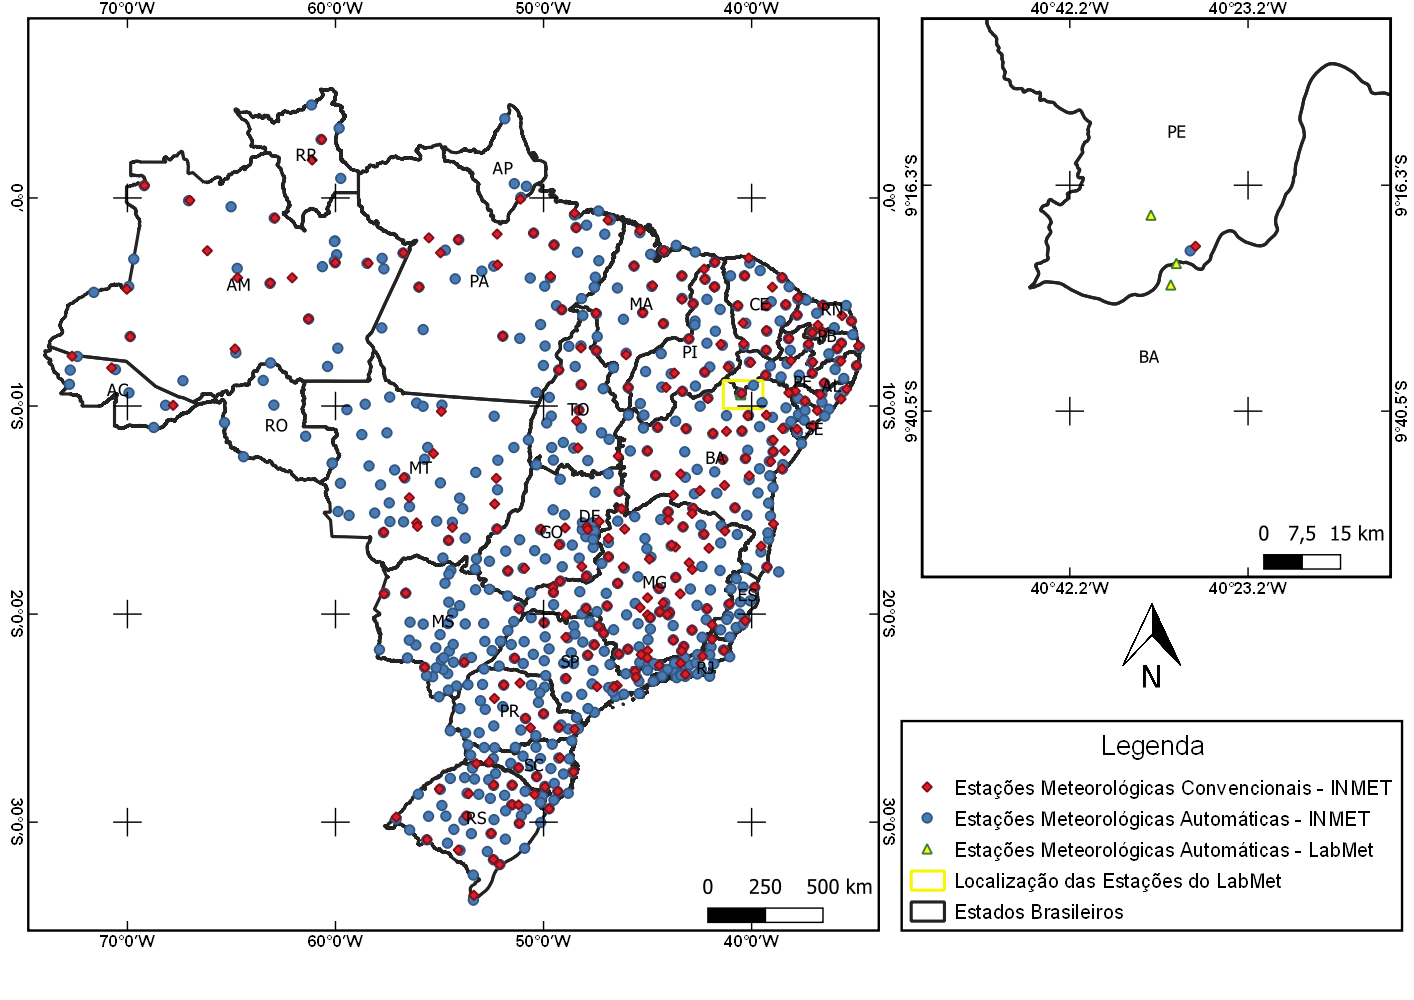
\includegraphics[width=0.9\textwidth]{figuras/espacializacao_estacoes.png}
    \label{figura_estacoes}
\end{figure}

\section{Coleta dos Dados das Estações Meteorológicas Convencionais do INMET}

Distribuídas ao longo de todo o território brasileiro, as estações meteorológicas convencionais vinculadas ao INMET representam os dados com maior série histórica dos três conjuntos, com observações que datam o ano de 1961. Ao todo, foram obtidas mais de 12 milhões de observações coletadas de todas as estações convencionais do INMET para o período de 1961 à 2019. Nas estações convencionais do INMET, cada observação corresponde à uma coleta realizada pelo observador em alguns momentos do dia. 

Os dados das estações convencionais do INMET foram baixados, de forma automatizada, em fevereiro de 2020 a partir do antigo portal do INMET\footnote{O antigo portal do INMET encontrava-se disponível, até a data do download dos dados, no endereço \href{http://www.inmet.gov.br}{http://www.inmet.gov.br}} utilizando a biblioteca Selenium \cite{salunke2014selenium}, versão 3.141.0. Desenvolvemos um script na linguagem de programação Python que percorreu cada uma das estações realizando o \textit{download}, em formato HTML, de todas as variáveis disponíveis na plataforma. A Tabela \ref{tab:variaveis_estacoes_convencionais} apresenta a lista das variáveis disponíveis nas estações convencionais.

\begin{table}[h!]
\caption{Variáveis disponíveis no conjunto de dados das estações meteorológicas convencionais do INMET.}
\label{tab:variaveis_estacoes_convencionais}
\begin{adjustbox}{width=\textwidth}
\begin{tabular}{|l|l|l|} % <-- Alignments: 1st column left, 2nd middle and 3rd right, with vertical lines in between
\hline
\textbf{Nome da coluna} & \textbf{Descrição} & \textbf{Unidade de Medida}\\
\hline
Estacao & Código da Estação  & - \\
\hline
Data & Data da Coleta do Dado  & DD/MM/YYYY\\
\hline
Hora & Hora da Coleta do Dado  & HHMM\\
\hline
Precipitacao & Precipitação Acumulada  & mm\\
\hline
TempBulboSeco  & Temperatura do Bulbo Seco & ºC\\
\hline
TempBulboUmido & Temperatura do Bulbo Úmido & ºC\\
\hline
TempMaxima  & Temperatura Máxima do Ar & ºC\\
\hline
TempMinima  & Temperatura Miníma do Ar & ºC\\
\hline
UmidadeRelativa  & Umidade Relativa do Ar & \% \\
\hline
PressaoAtmEstacao  & Pressão Atmosférico no Nível da Estação & mbar \\
\hline
PressaoAtmMar  & Pressão Atmosférico no Nível do Mar & mbar \\
\hline
DirecaoVento  & Direção do Vento & Código INMET\\
\hline
VelocidadeVento  & Velocidade do Vento & m/s\\
\hline
Insolacao  & Insolação & horas\\
\hline
Nebulosidade & Nebulosidade & décimos \\
\hline
Evaporacao Piche & Evaporação de Piche & mm\\
\hline
Temp Comp Media & Temperatura Compensada Média & ºC\\
\hline
Umidade Relativa Media & Umidade Relativa Média do Ar & \% \\
\hline
Velocidade do Vento Media & Velocidade Média do Vento & m/s\\
\hline
\end{tabular}
\end{adjustbox}
\end{table}

\section{Coleta dos Dados das Estações Meteorológicas Automáticas do INMET}

O segundo conjunto de dados utilizados foram obtidos das estações meteorológicas automáticas vinculadas ao INMET, assim como as convencionais, distribuídas por todo o território nacional. Diferente das estações convencionais que possuem três observações ao longo do dia, e dados desde de 1961, as estações automáticas do INMET coletam dados a cada uma hora desde o ano de 2000. Ao todo, obtivemos quase 55 milhões de observações coletadas de todas as 610 estações meteorológicas automáticas do INMET, para o período de 2000 à 2019.

Os dados de cada uma das estações automáticas foram baixados em agosto de 2020 diretamente do novo portal do INMET\footnote{O novo portal do INMET encontrava-se disponível, até a data do download dos dados, no endereço \href{https://portal.inmet.gov.br/}{https://portal.inmet.gov.br/}} em formato CSV. A Tabela  \ref{tab:variaveis_estacoes_automaticas} apresenta a lista das variáveis disponíveis nos dados baixados.

\begin{table}[h!]
\caption{Variáveis disponíveis no conjunto de dados das estações meteorológicas automáticas do INMET}
\label{tab:variaveis_estacoes_automaticas}
\begin{adjustbox}{width=\textwidth}
\begin{tabular}{|l|l|l|}
\hline
\textbf{Nome da coluna} & \textbf{Descrição} & \textbf{Unidade de Medida}\\
\hline
ESTACAO & Código da Estação  & -\\
\hline
DATA (YYYY-MM-DD) & Data da observação  & YYYY-MM-DD\\
\hline
HORA (UTC) & Hora da observação  & HH\\
\hline
PRECIPITACAO TOTAL HORARIO (mm) & Precipitação Acumulada  & mm\\
\hline
PRESSAO ATMOSFERICA AO NIVEL DA ESTACAO, HORARIA (mB)  & Pressão Atmosférica Instantânea no Nível da Estação & ºC\\
\hline
PRESSAO ATMOSFERICA MAX.NA HORA ANT. (AUT) (mB) & Pressão Atmosférica Máxima & mbar\\
\hline
PRESSAO ATMOSFERICA MIN. NA HORA ANT. (AUT) (mB)  & Pressão Atmosférica Mínima & mbar\\
\hline
RADIACAO GLOBAL (W/m2)  & Radiação Sola Global & W/m2\\
\hline
TEMPERATURA DO AR - BULBO SECO, HORARIA (C)  & Temperatura do Bulbo Seco & ºC \\
\hline
TEMPERATURA DO PONTO DE ORVALHO (C)  & Pressão Atmosférico no Nível da Estação & mbar \\
\hline
PEMPERATURA MAXIMA NA HORA ANT. (AUT) (C)  & Pressão Atmosférico no Nível do Mar & mbar \\
\hline
TEMPERATURA MINIMA NA HORA ANT. (AUT) (C)  & Direção do Vento & Código INMET\\
\hline
TEMPERATURA ORVALHO MAX. NA HORA ANT. (AUT) (C)  & Velocidade do Vento & m/s\\
\hline
TEMPERATURA ORVALHO MIN. NA HORA ANT. (AUT) (C)  & Insolação & horas\\
\hline
UMIDADE REL. MAX. NA HORA ANT. (AUT) (\%) & Nebulosidade & décimos \\
\hline
UMIDADE REL. MIN. NA HORA ANT. (AUT) (\%) & Evaporação de Piche & mm\\
\hline
UMIDADE RELATIVA DO AR, HORARIA (\%) & Temperatura Compensada Média & ºC\\
\hline
VENTO, DIRECAO HORARIA (gr) & Umidade Relativa Média do Ar & \% \\
\hline
VENTO, RAJADA MAXIMA (m/s) & Velocidade Média do Vento & m/s\\
\hline
VENTO, VELOCIDADE HORARIA (m/s) & Velocidade Média do Vento & m/s\\
\hline
\end{tabular}
\end{adjustbox}
\end{table}

\section{Coleta dos Dados das Estações Meteorológicas Automáticas do LabMet}

O último conjunto de dados utilizado foi obtido de 3 estações meteorológicas automáticas localizadas no Vale do Rio São Francisco, entre os estados da Bahia e Pernambuco. Estas estações são administradas pelo Laboratório de Meteorologia da Universidade Federal do Vale do São Francisco (LabMet), que disponibiliam dados diário das estações através de seu portal\footnote{O portal do LabMet encontrava-se disponível, até a data de agosto de 2020, no endereço \href{http://labmet.univasf.edu.br}{http://labmet.univasf.edu.br}}. Ao todo, baixamos, em formato XLS, mais de 11 mil registros disponibilizados para as três estações automáticas entre o período de 2007 à 2020. A Tabela \ref{tab:estacoes_automaticas_labmet} descreve as variáveis contidas no conjunto de dados. 

\begin{table}[h!]
\caption{Descrição dos campos/colunas dos datasets.}
\label{tab:estacoes_automaticas_labmet}
\begin{tabular}{|l|l|l|}
\hline
\textbf{Nome da coluna} & \textbf{Descrição} & \textbf{Unidade de Medida}\\
\hline
Estacao & Código gerado como identificar da estação & - \\
\hline
Data & Data da observação & YYYY-MM-DD\\
\hline
temperatura & Temperatura média do ar & ºC\\
\hline
temperatura maxima & Temperatura máxima do ar & ºC\\
\hline
temperatura minima & Temperatura mínima do ar & ºC\\
\hline
umidade & Umidade relativa média do ar & \% \\
\hline
umidade maxima & Umidade relativa máxima do ar & \% \\
\hline
umidade minima & Umidade relatima mínima do ar & \% \\
\hline
vento maxima 10m & Velocidade máxima do vento diária  & m/s \\
\hline
rad. solar global & Radiação solar global  & MJ/m$^2$/dia\\
\hline
evap. de referencia & Evapotranspiração de Referência & mm/dia\\
\hline
\end{tabular}
\end{table}